% !TEX TS-program = pdflatex
% !TEX encoding = UTF-8 Unicode
% !TEX root = ../main.tex
% !TEX spellcheck = en-US
% ****************************************************************************************
% File: methods.tex
% Author: Jakob Spindler
% Date: 2024-10-16
% ****************************************************************************************
\chapter{Methods}
\label{chapter:methods}

\section{Controller Design}
\label{section:controller_design}

The PLECS model of the converter includes the following:
\begin{itemize}
    \item a PID controlled duty cycle
    \item a noise source for the input voltage
    \item a variable load
\end{itemize}

all of which can be selected to be active or inactive as can be seen in \autoref{fig:PLECS_model} and \autoref{fig:PLECS_subsystems}.

\begin{figure}[htbp]
    \centering
    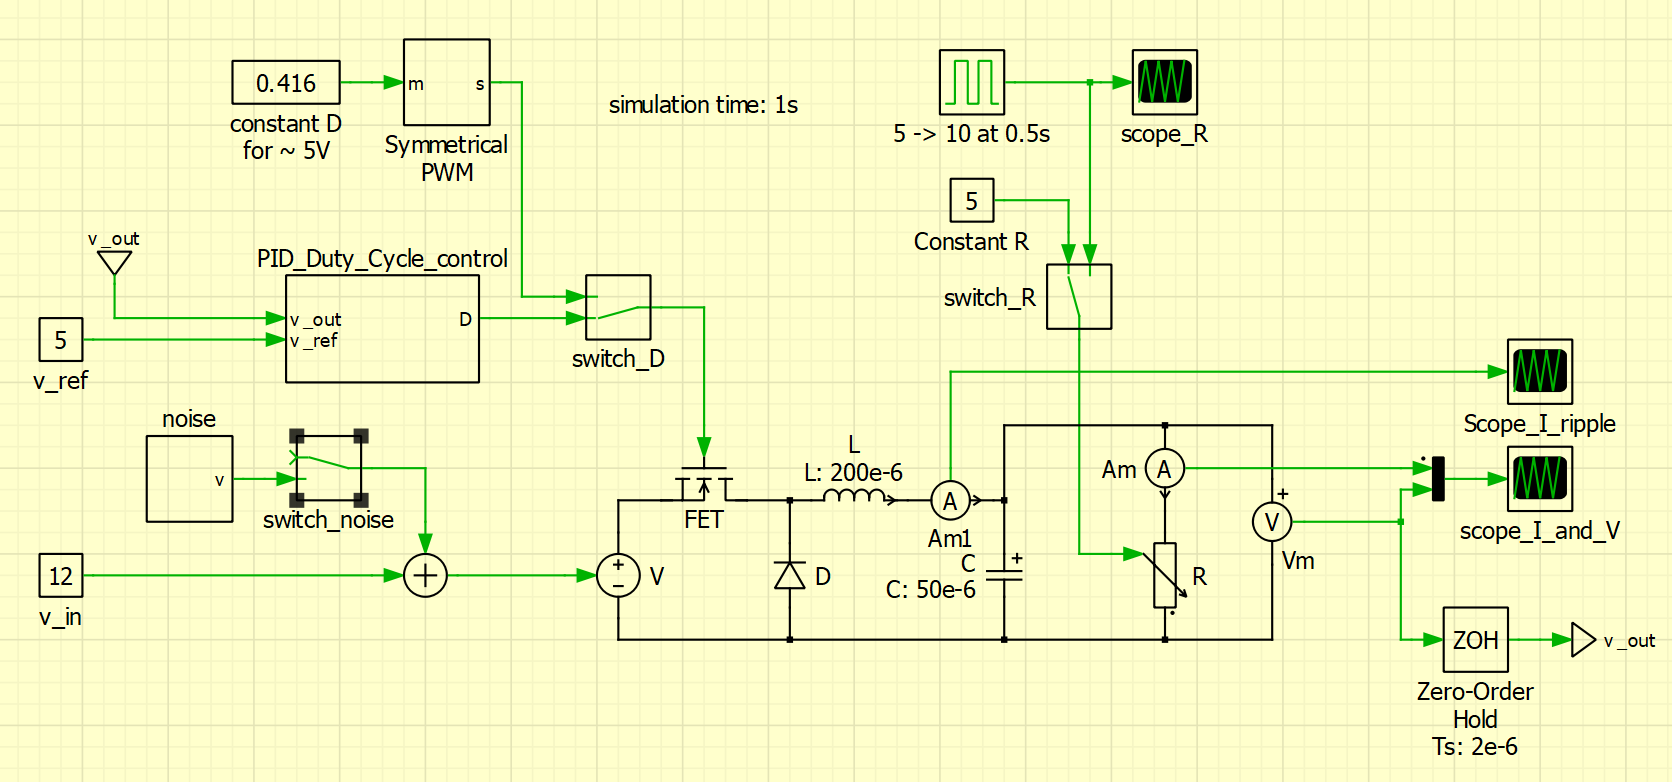
\includegraphics[width=0.95\textwidth]{img/PLECS_model_full_view.png}
    \caption{PLECS model of the Buck-Converter}
    \label{fig:PLECS_model}
\end{figure}

\begin{figure}[htbp]
    \centering
    \begin{subfigure}[b]{0.55\textwidth}
        \centering
        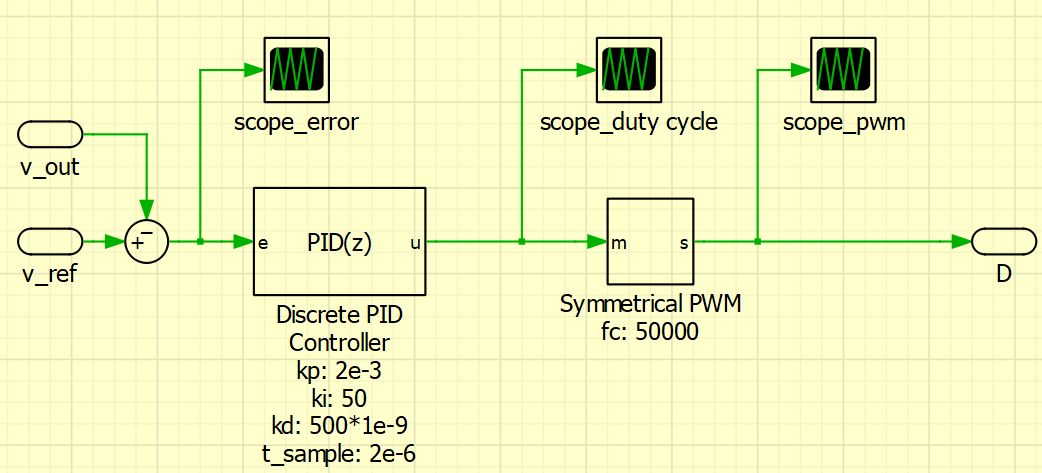
\includegraphics[width=\textwidth]{img/PLECS_PID_Duty_Cycle_control.png}
        \caption{PLECS model of the PID\_Duty\_Cycle\_control subsystem}
        \label{fig:PLECS_PID}
    \end{subfigure}
    \hfill
    \begin{subfigure}[b]{0.40\textwidth}
        \centering
        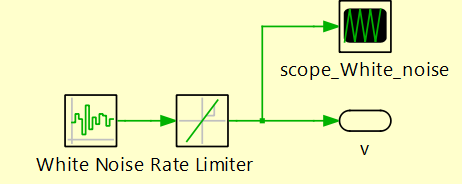
\includegraphics[width=\textwidth]{img/PLECS_noise.png}
        \caption{PLECS model of the noise subsystem}
        \label{fig:PLECS_noise}
    \end{subfigure}
    \caption{PLECS model subsystems}
    \label{fig:PLECS_subsystems}
\end{figure}

\begin{figure}[htbp]
    \centering
    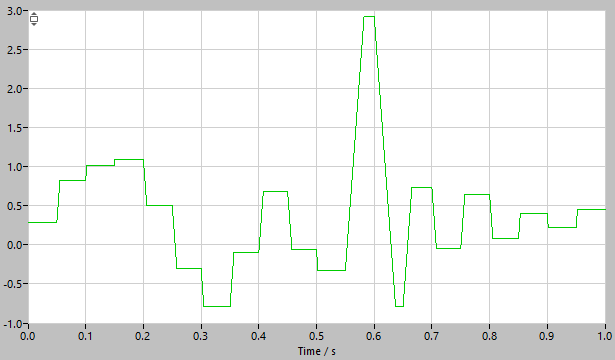
\includegraphics[width=0.8\textwidth]{img/noise.png}
    \caption{White noise with a standard deviation of \qty{1}{\volt} and a sample time of \qty{50}{\milli\second}}
    \label{fig:noise}
\end{figure}

The control of the converter was tested under the following conditions and compared to the behaviour of the converter with a fixed duty cycle:
\begin{itemize}
    \item noise on the input voltage (white noise with a standard deviation of \qty{1}{\volt} and a sample time of \qty{50}{\milli\second} as seen in \autoref{fig:noise})
    \item a load step from \qty{5}{\ohm} to \qty{10}{\ohm} at \qty{0.5}{\second}
    \item startup behaviour
\end{itemize}

\section{Hardware-in-the-Loop (HIL) Setup}
\label{section:hil_setup}

As a next step, the controller-converter system shown in \autoref{section:controller_design} is split into two distinct discrete subsystems that can be used for code generation for the respective hardware and each form the controller and converter respectively. The blocks are connected using real-time interface blocks, like the \textit{Analog In (triggered)} and \textit{PWM} blocks for the Controller and the \textit{Analog Out1} and \textit{PWM Capture1} blocks for the Converter. The generic HIL setup is shown in \autoref{fig:HIL_setup}. The subsystems are then connected into a closed control loop with a scope block to monitor the output of the converter.

\begin{figure}[htbp]
    \centering
    % Top figure
    \begin{subfigure}[b]{0.9\textwidth}
        \centering
        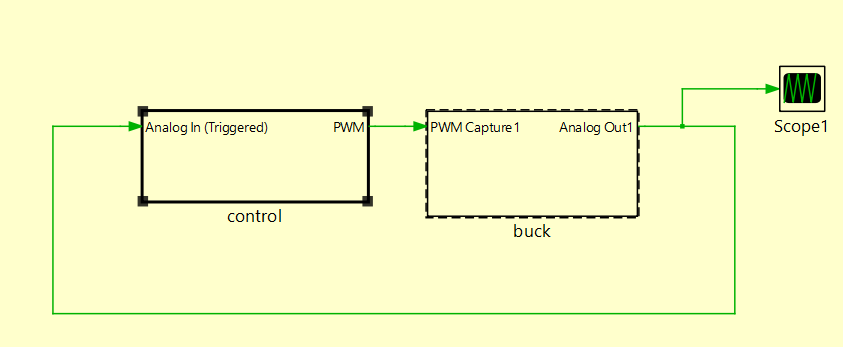
\includegraphics[width=\textwidth]{img/HIL/generic_setup.png}
        \caption{PLECS Model of the generic HIL setup}
        \label{fig:plecs_model_generic_hil}
    \end{subfigure}

    % Bottom row figures
    \begin{subfigure}[b]{0.49\textwidth}
        \centering
        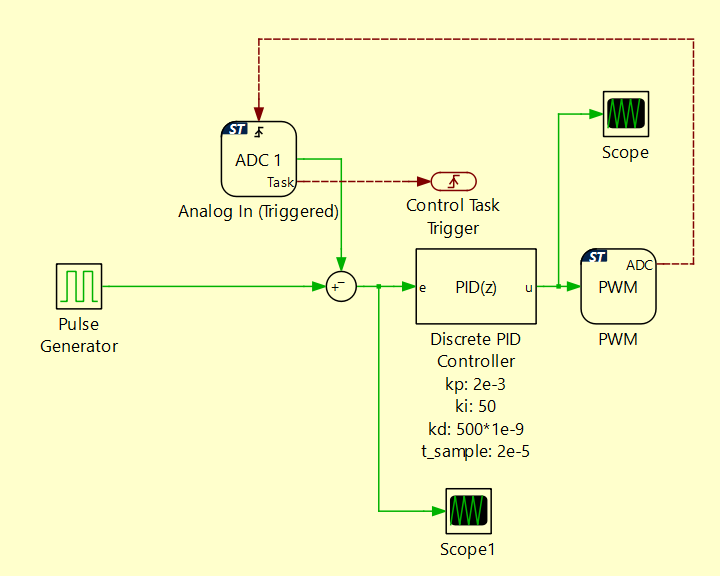
\includegraphics[width=\textwidth]{img/HIL/generic_control.png}
        \caption{Controller Subsystem}
        \label{fig:generic_controller}
    \end{subfigure}
    \hfill
    \begin{subfigure}[b]{0.49\textwidth}
        \centering
        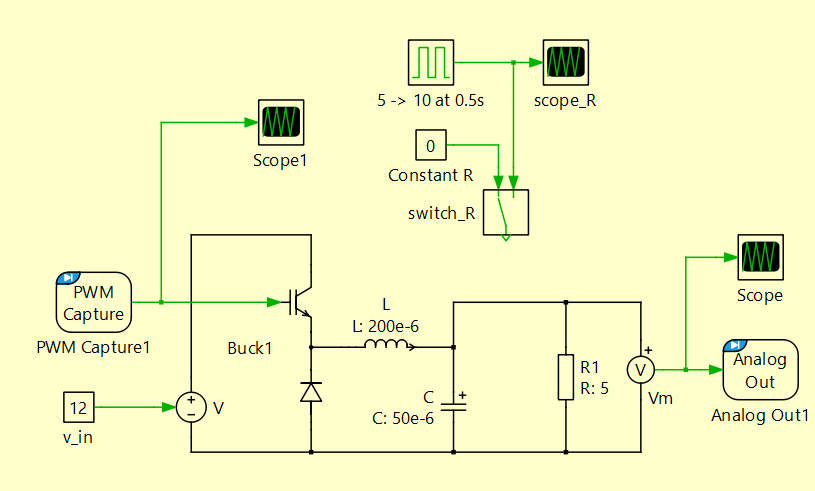
\includegraphics[width=\textwidth]{img/HIL/generic_buck.png}
        \caption{Buck Converter Subsystem}
        \label{fig:generic_buck}
    \end{subfigure}

    \caption{PLECS Generic HIL Setup and Subsystems}
    \label{fig:HIL_setup}
\end{figure}

\subsection{Verification of the Sampling Frequencies}
\label{subsection:sampling_frequencies}

Before actual hardware implementation, it is advisable to verify that the whole system still operates as inteded with descretization parameters for the subsystems set.
As a rule of thumb, the sample frequency of the controller may equal the switching frequency of the converter, while the sample frequency of the converter may be set to a multiple of the switching frequency, ideally 10 to 20 times the switching frequency.

This verification can easily be done withoput hardware by setting the desired sampling frequencies and then generating code for the subsystems with a generic target -- thus enabling code execution on the local machine. By inspecting the output of the converter, a statement can be made about the correct operation of the system.

For simplicity reasons, a reference-voltage-pulse of \qty{10}{\hertz} with a duty cycle of \qty{50}{\percent} and amplitudes of \qty{5}{\volt} and \qty{10}{\volt} was used as the input signal for the controller.
The sampling frequencies were chosen as
\begin{itemize}
    \item $f_{sw}$ for the controller
    \item $10f_{sw}$ for the buck converter
\end{itemize}
The output of the converter is shown in \autoref{fig:verification}.
\begin{figure}[htbp]
    \centering
        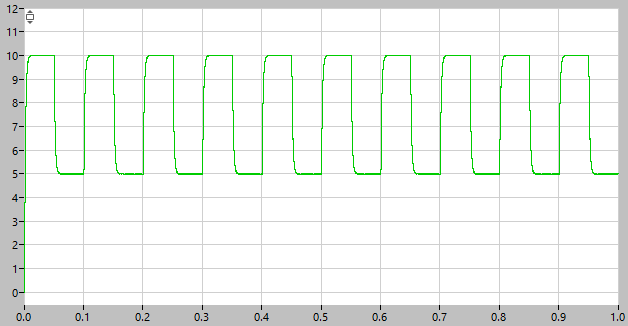
\includegraphics[width=0.8\textwidth]{img/HIL/generic_v_out.png}
    \caption{Buck converter output voltage -- Verification of the HIL setup with local code execution}
    \label{fig:verification}
\end{figure}

\subsection{Hardware Implementation}
\label{subsection:hardware_implementation}
With the verification of the sampling frequencies, the next step is to generate code for the respective hardware.


The controller is implemented on an STM32G4 microcontroller, while the buck converter is implemented on a PLECS RT-Box. The hardware setup is shown in \autoref{fig:hardware setup}.

\pgfplotsset{compat=1.18}
\begin{figure}[htbp]
    \centering
    \begin{adjustbox}{max width=0.8\textwidth}
        \begin{circuitikz}
    \tikzstyle{every node}=[font=\large]
    \draw  (10,18.5) rectangle  node {\LARGE RT Box} (15,14.75);
    \draw  (21.25,18.5) rectangle (27.5,14.75);
    \draw (11.25,14.75) to (11.25,13.75) node[ground]{};
    \draw (26.25,14.75) to (26.25,13.75) node[ground]{};
    \draw (20.25,19.75) to (20.25,19.5) node[ground]{};
    \draw [->, >=Stealth] (15,17.75) -- (21.25,17.75)node[pos=0.5, fill=white]{$v_{out}/5$};
    \draw [->, >=Stealth] (21.25,15.75) -- (15,15.75)node[pos=0.5, fill=white]{PWM};
    \node [font=\large] at (22.5,17.75) {Analog In 2};
    \node [font=\large] at (22.75,15.75) {B9 -TIM8, Ch3};
    \node [font=\LARGE] at (24,16.75) {STM32G4};
    \node [font=\large] at (13.75,15.75) {Digital In 7};
    \node [font=\large] at (13.75,17.75) {Analog Out 2};
    \node at (15.5,17.75) [circ] {};
    \node at (16.25,15.75) [circ] {};
    \draw (15.5,17.75) to[short] (15.5,21);
    \draw (16.25,15.75) to[short] (16.25,20.25);
    \draw  (20.25,21.25) circle (1.5cm);
    \draw [->, >=Stealth] (15.5,21) -- (18.75,21);
    \draw [->, >=Stealth] (16.25,20.25) -- (19.25,20.25);
    \draw [short] (19.25,21) -- (20.75,21.75);
    \draw [short] (20.75,21.75) -- (20.75,21);
    \draw [short] (20.75,21) -- (21.25,21);
\end{circuitikz}
    \end{adjustbox}
    \caption{Hardware setup schematic}
    \label{fig:hardware setup}
\end{figure}


% EOF